\section{Introducción a la ingeniería de software}

Segun wikipedia, se define Software como:

\begin{enfasis}
    El ``sistema formal'' de un sistema informático, que comprende el conjunto de los componentes lógicos necesarios
    que hace posible la realización de tareas específicas, en contraposición a los componentes físicos que son 
    llamados hardware.
\end{enfasis}

Para hacerlo más sencillo de entender, pero sin perder ningun tipo de detalle, para nosotros Software será:

\begin{center}
    \textbf{Los programas y toda la información asociada y materiales necesarios para soportar su instalación, 
    operación, reparación y mejora.}
\end{center}

Por tanto el software ya no tiene por que ser simplemente un programa de Java, o quizas Python, que se ejecuta 
(como los creados en asignaturas anteriores), sino que tambien puede ser un sistema formado por uno o varios 
programas, y otra gran cantidad de elementos, sean DBMS, ficheros, etc.

\noindent Siendo específicos, para crear un Software necesitaremos:
\begin{enumerate}
    \item Detallar las especificaciones.
    \item Diseñar la solución.
    \item Codificar los algoritmos.
    \item Probar el programa (o sistema).
    \item Documentar
    \item Mantener
\end{enumerate}
\noindent Esta serie de pasos es lo que se conoce como \textbf{ciclo de vida} del Software, el cual (como bien 
indica su nombre) se ``reinicia'' interminablemente durante la existencia del programa o sistema.

\noindent\rule{\textwidth}{0.4pt}

Antes de seguir indagando en los aspectos ``técnicos'' del Software, y para reflejar la importancia y complejidad 
que puede llegar a alcanzar el Software, hablemos en términos económicos y de lineas de código\dots

Segun datos de la BSA (\textit{Bussines Software Alliance}) del 2007:
\begin{itemize}
    \item El Software recoge alrededor de $1'7$ millones de empleos en EEUU.
    \item Contribuye en más de $297.000$ millones de dólares al PIB de el mismo.
    \item Tiene un crecimiento por encima del $14\%$ (¿anual?)
    \item Se invierten unos $43.000$ millones de dólares en I+D.
    \item Existen cerca de $90.000$ patentes relacionadas con el Software.
    \item Recoge un mercado de $297.000$ millones de dólares, $80.000$ millones de ellos para PC.
\end{itemize}

En la siguiente tabla se pueden observar algunos ejemplos de Software y las lineas de código que lo componen,
que a pesar de no ser totalmente lineal al tamaño del mismo (en cuanto a complejidad, inversión económica o cantidad
de personas trabajando en el), nos puede dar una idea de los monstruos con los que se trabajan:
\begin{table}[h]
    \centering
    \begin{tabular}{cc}
        \hline
        Proyecto        & \textit{LOC} (millones)   \\
        \hline
        Windows NT 3.1  & 4-5                       \\
        Windows XP      & 40                        \\
        \hline
        Linux 2.6.0     & 5.2                       \\
        Linux 2.6.35    & 13.5                      \\
        \hline
        Debian 3.0      & 104                       \\
        Debian 5.5      & 324                       \\
        \hline
        Mac OS X 10.4   & 86                        \\
        \hline
    \end{tabular}
\end{table}

\small\textit{Si, lo se, los ejemplos suenan a prehistoria, si te molesta mucho cambialos tu mismo, que a mi me da
mucha pereza actualizarlos. Buena suerte\dots}

\vspace*{2mm}

Otra posible forma de entender la magnitud de la importancia de un \textbf{buen} Software son los siguientes 
ejemplos de noticias reales:

\begin{enumerate}
    \item Recuperados $2.000$ de las $15.000$ pruebas radiológicas que se perdieron en el Hospital de Ávila
    (\href{https://www.elnortedecastilla.es/avila/201602/01/recuperados-pruebas-radiologicas-perdieron-20160201193859.html}{Fuente: El Norte de Castilla}).

    Como dijo Felix en clase, esto no se trata de los $2.000$ recuperados, se debería tratar de los otros $13.000$
    perdidos. Un fallo en el Software que gestionaba estos datos provocó pérdidas económica y humanas dificiles de 
    calcular.

    \item El Boeing 737 MAX y sus dos accidentes fatales en menos de 5 meses encienden las alertas en la aviación 
    comercial (\href{https://www.xataka.com/vehiculos/avion-boeing-737-max-sus-dos-accidentes-fatales-cinco-meses-encienden-alertas-aviacion-comercial}{Fuente: Xataca}).

    De nuevo, un fallo de Software en el sistema anti pérdidas del Boeing 737 MAX provoca pérdidas millonarias y 
    cientos de muertos por incompetencia a la hora de desarrollar Software (en este caso, se habla de que Boeing
    pudo estar pagando menos que el sueldo mínimo interprofesional a sus desarrolladores, ¡menuda ganga!). 
\end{enumerate}

\noindent Queda más que evicenciada la crucial importancia de la ingeniería de Software y las buenas prácticas que
la rodean.

\noindent\rule{\textwidth}{0.4pt}

Por supuesto que estamos de acuerdo en que el Hardware se desgasta, una bombilla se puede fundir, un condensador puede
explotar, quemar, o cualquier otra exagerada desdicha. Pero ocurre que el Software también se degrada, ¿cómo puede
ser? Una evaluación lógica, por ejemplo, \lstinline{if (numero > 0) then ...}, siempre se comportará igual, ¿no? %TODO modo code

\vspace*{2mm}

Pues no tiene por que. Una característica intrinseca al Software es que se actualiza, y muy rápidamente. Por tanto,
cosas que en el pasado funcionaban, aunque no hayan sido modificadas explicitamente, implicitamente se pueden ver
afectadas por modificaciones ajenas. A esto se le llaman habitualmente efectos secundarios.

\newpage

Es donde surje aquí el concepto de versión. Para continuar adaptandose y expandiendose a las necesidades, el
Software se actualiza al una nueva versión, maximizando las probabilidades de fallos en cada cambio.

\begin{figure}[h]
    \centering
    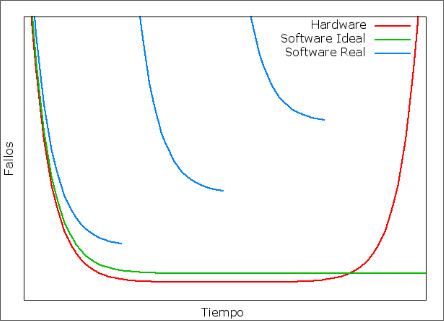
\includegraphics[width=0.7\textwidth]{assets/SoftwareFails.jpeg}
    \caption{Gráfico que ilustra el suceso}
    \label{graph:softwarefails}
\end{figure}

Vistas toda la infinidad de cosas malas que pueden ocurrir con un \textbf{mal} Software, definiremos lo que si es
\textbf{buen} Software. Los atributos de un buen producto Software son:

\begin{enumerate}
    \item \textbf{Mantenibilidad}. Es la posibilidad del Software de evolucionar para adaptarse a las necesidades
    de cambio de los clientes. Una definición más exhaustiva puede ser la siguiente
    \begin{enfasis}
        Esta característica representa la capacidad del producto Software para ser modificado efectiva y
        eficientemente, debido a necesidades evolutivas, correctivas, correctivas o perfectivas.
    \end{enfasis}
    No tener cuidado de hacer un Software \textbf{mantenible} provoca lo que se conoce como \textit{Deuda Técnica}.
    Puedes investigar más sobre ello en su entrada de \href{https://es.wikipedia.org/wiki/Deuda_t%C3%A9cnica}{wikipedia}.
    \item \textbf{Confiabilidad}. El Software no debe causar daños físicos o económicos en caso de fallo del sistema
     o un comportamiento inesperado. Esto implica la \textbf{Fiabilidad}, \textbf{Seguridad} y \textbf{Protección}. \\
     Por tanto no es solo que el Software no deba fallar, también es importante que \textit{no pueda saberse} que
     tiene estos fallos, para poder proteger su integridad frente a ataques maliciosos.
     \item \textbf{Eficiencia}. No deben malgastarse recursos del sistema. Hacer un Software poco eficiente no solo
     te hace mal Ingeniero, también te va a hacer más pobre; los recursos son dinero.
     \item \textbf{Usabilidad}. Con este termino surje una cuestión interesante, pues es muy loable la pregunta...
     \textit{¿Qué es usable, y qué no?} Pues \textbf{depende}. \\
     Definiremos usabilidad como el Software que \textbf{fácil de usar} y que ofrece una \textbf{interfaz de usuario
     apropiada} y \textbf{documentación adecuada}. Por lo tanto lo usable depende en gran medida de a quien se le 
     ofrece el Software, pues para un Ingeniero Informático hecho y derecho le puede parecer muy usable Vi 
     (Vim, NVim) pero a duras penas sacará buen provecho de, por ejemplo, Tinder.
\end{enumerate}

\newpage

Ya se ha mencionado anteriormente que un \textbf{Sistema Software} ya no es simplemente un código, sino un conjunto
de muchas cosasa trabajando a la vez. Pero qué cosas, cómo trabajan, porqué no un programa y ya está (nos quieren
hacer la vida imposible estos informáticos del diablo). Bien, pues paso a paso.

\noindent Empezaremos definiendo correctamente lo que es un \textbf{Sistema}:

Un \textbf{Sistema Software} es un conjunto de elementos interrelacionados que trabajan conjuntamente para
cumplir algún objetivo. Algunas características notables de los sistemas es que tienen \textit{propiedades
emergentes} (yo tampoco se lo que significa)\footnote{En teoría de sistemas, las propiedades emergentes son 
atributos que surgen del funcionamiento de un sistema y que no se pueden identificar en las propiedades de los
componentes que forman el mismo. \href{https://www.alegsa.com.ar/Dic/propiedad_emergente.php}{Fuente: Alegsa}}
diferentes de las de sus elementos y que los sistemas que incluyen personas son \textit{no deterministas}, pues
la acción de los humanos no lo es, y se ven afectados por ella.

Podemos distinguir entre 3 tipos de sistemas

\begin{enumerate}
    \item Sistemas físicos. Transforman un flujo de entrada en uno de salida.
    \item Sistemas de gestión. Controlan los sistemas físicos decidiendo el comportamiento de los mismos en función
    de los objetivos marcados.
    \item Sistemas de información. Comunican sistemas físicos con los de gestión.
\end{enumerate}

Por fin sabemos lo que es un Software, lo que es un sistema, los criterios de bondad del Software y todas esas
cosas que hemos dicho que debe hacer un Ingeniero. ¿Pero Ingeniero de qué? Pues Ingeniero de Software\dots

La Ingeniería de Software se define como

\begin{enfasis}
    La aplicación de un enfoque \textbf{sistemático}, \textbf{disciplinado} y \textbf{cuantificable} hacia el
    desarrollo, operación y mantenimiento del Software; es decir, la aplicación de la ingeniería al Software

     Estándar $610.12$ IEEE
\end{enfasis}

Desde distintos puntos de vista:
\begin{enumerate}
    \item Diseño, construcción y mantenimiento de grandes sistemas software
    \item Construcción multi-persona de software multi-versión
    \item Conjunto de técnicas que se enfrentan al software como un producto de ingeniería que requiere 
    planificación, análisis, diseño, implementación pruebas y mantenimiento
    \item Aplicación disciplinada de los principios y métodos de la ingeniería, la ciencia y las matemáticas para
    la producción económicamente rentable de software de calidad
    \item Conjunto de teorías, métodos y herramientas para el desarrollo profesional de software
\end{enumerate}

Esto está textualmente copiado de las transparencias de clase, por que lo vi importante y tampoco sabía que más
añadir, pero creo que deja más que claro lo que es, ¿no? Pero somo hemos dicho lo que es, falta explicar en que
consiste

La Ingeniería de Software es una actividad de \textbf{modelado}. El modelado implica conocer a la perfección un
problema para tener la capacidad de explicarlo con máximo detalle en un ``lenguaje'' que permita interpretarlo ya
resolverlo (esta interpretación es mía, no algo que haya que aprenderse de pe a pa).